\section{Experimentación} \label{sec:experimentacion}

En esta sección pondremos a prueba a ambos Ray Tracer, y los compararemos entre
sí en diferentes escenarios para ver si efectivamente el uso de instrucciones
SIMD mejora el rendimiento de los mismos.

Todos los experimentos se corrieron en una notebook HP 14-dk1003dx, que cuenta
con una CPU AMD Athlon Silver 3050U de 2.3GHz, 1MB de cache L2, y 16GB de RAM.
El sistema corre Arch Linux, y utiliza la versión 6.7.5 de linux. Los binarios
en C y en ASM se compilaron con GCC v13.2.1 y con NASM v2.16.01 respectivamente.

\subsection{Diferencia entre implementaciones}

En este primer experimento, generaremos imágenes para escenas similares usando
las distintas implementaciones que tenemos a disposición: RTMongi, RTC++, y
RTASM (ignoramos RTC, ya que genera exactamente las mismas imágenes). La
motivación es tener una idea general de cómo se diferencian los ray tracers, y
además una medida del tiempo que tarda cada uno en generar la imagen.

Por cómo está implementado cada uno, esperamos que RTMongi sea el más rápido, y
RTC++ el más lento. La implementación de Mongi usa una simplificación para el
cálculo del color, en vez de ``rebotar'' el rayo por la escena hasta llegar a
una fuente de luz y combinar los aportes de todas las intersecciones, se calcula
el aporte de cada fuente de luz al primer punto de intersección del rayo.

\begin{figure}[H]
  \centering
  \begin{subfigure}[b]{0.45\textwidth}
    \centering
    \includegraphics[width=\textwidth]{../images/impl_diffs/mongi-sphere.png}
    \caption{Implementación de Mongi}
    \label{fig:yellow-sphere-mongi}
  \end{subfigure}
  \hfill
  \begin{subfigure}[b]{0.45\textwidth}
    \centering
    \includegraphics[width=\textwidth]{../images/impl_diffs/asm-sphere.png}
    \caption{Implementación en ASM}
    \label{fig:yellow-sphere-asm}
  \end{subfigure}
  \hfill
  \begin{subfigure}[b]{0.45\textwidth}
    \centering
    \includegraphics[width=\textwidth]{../images/impl_diffs/cpp-sphere.png}
    \caption{Implementación original en C++}
    \label{fig:yellow-sphere-cpp}
  \end{subfigure}

  \caption{Escena de una esfera amarilla sobre una superficie gris}
  \label{fig:yellow-sphere}
\end{figure}

En la figura \ref{fig:yellow-sphere} podemos ver las imágenes generadas. La de
Mongi (\ref{fig:yellow-sphere-mongi}) es claramente distinta por lo que ya
explicamos anteriormente, se puede ver como tanto el ángulo de incidencia, como
la distancia de la intersección a la luz afectan a su aporte en la imagen,
haciendo que algunas partes se vean más oscuras. Por otro lado, las
implementaciones en ASM (\ref{fig:yellow-sphere-asm}) y en C++
(\ref{fig:yellow-sphere-cpp}) generan imágenes muy parecidas, y más iluminadas
que en la primera imagen.

La diferencia de color que se puede apreciar entre estas últimas se debe a cómo
están iluminadas. En RTASM usamos un plano a cierta altura para que simule una luz
solar, mientras que en RTC++ los rayos que no colisionan con ningún objeto toman
un color predeterminado que depende de su dirección.

Los tiempos de ejecución los obtenemos realizando 10 mediciones y tomando el
promedio. Usamos el comando \texttt{time} que se puede encontrar en la mayoría de
distribuciones de Linux. El tiempo CPU es el tiempo que el programa estuvo
ejecutando, mientras que el Real es el tiempo real que transcurrió desde que
empezó la ejecución hasta que termino (puede incluir esperas de IO,
manejo de interrupciones, etc.)

\begin{table}
  \centering
  \begin{tabular}[t]{l l l l}
    Tiempo (ms.) & \vline~RTMongi & RTASM  & RTC++   \\
    \hline
    CPU          & \vline~328.4   & 4326.8 & 14986.5 \\
    Real         & \vline~365.3   & 4361.8 & 15052.3 \\
  \end{tabular}
  \caption{Tiempos de ejecución de cada implementación}
  \label{tbl:impl-time-diff}
\end{table}

Como podemos ver, los resultados concuerdan con nuestras suposiciones iniciales.
Mongi es casi 13 veces más rápido que ASM, y ASM 3.5 veces más rápido que C++.

Si bien la diferencia es sustancial, es importante recordar que los RTASM y
RTC++ pueden parametrizar opciones como \texttt{spp} y \texttt{max\_depth},
mientras que RTMongi los tiene fijados en 1 por definición. Si corremos
nuevamente RTASM, pero con un \texttt{spp=1} y \texttt{max\_depth=5}, podemos obtener un
tiempo de ejecución de 350 ms sacrificando la calidad de la imagen.

\subsection{Ciclos de clock para distintas resoluciones en escena preparada}

Inspirado en el experimento realizado por Mongi en su trabajo, compararemos los
tiempos de ejecución de RTC y RTASM para una misma escena, pero variando la
resolución de la imagen de salida. Se espera que RTASM sea ampliamente superior
a RTC en este aspecto.

\begin{figure}[H]
  \centering
  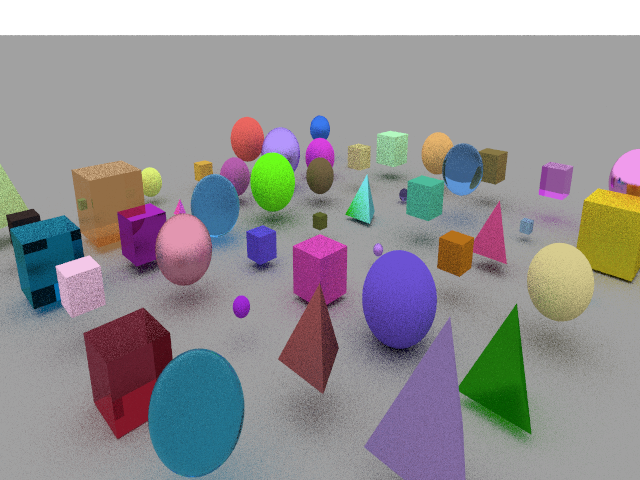
\includegraphics[width=.8\textwidth]{./imgs/exp2-scene.png}
  \caption{Escena a utilizarse para la medición}
  \label{fig:exp2-scene}
\end{figure}

Usaremos la escena que se muestra en la figura \ref{fig:exp2-scene} para
realizar las mediciones usando las opciones \texttt{-m 1 -n 3} del programa, que
le indica realizar 3 mediciones de tipo 1 (cantidad de ciclos de clock), y
obtener el promedio.

\begin{figure}[H]
  \centering
  \begin{subfigure}[b]{0.45\textwidth}
    \centering
    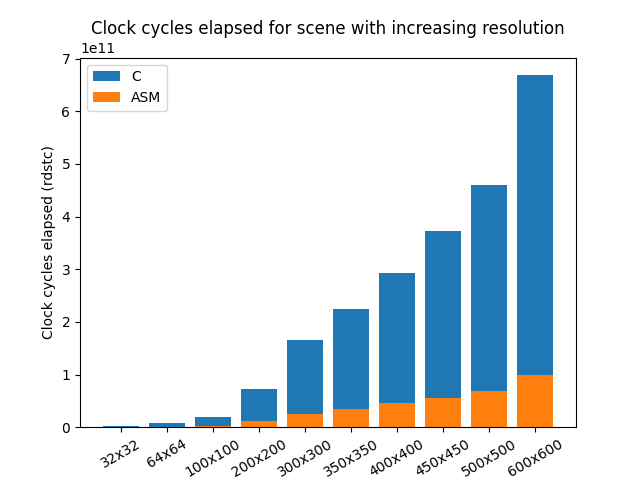
\includegraphics[width=\textwidth]{./imgs/exp2-res-bar.png}
    \caption{Ciclos de clock por resolución}
    \label{fig:exp2-res-bar}
  \end{subfigure}
  \hfill
  \begin{subfigure}[b]{0.45\textwidth}
    \centering
    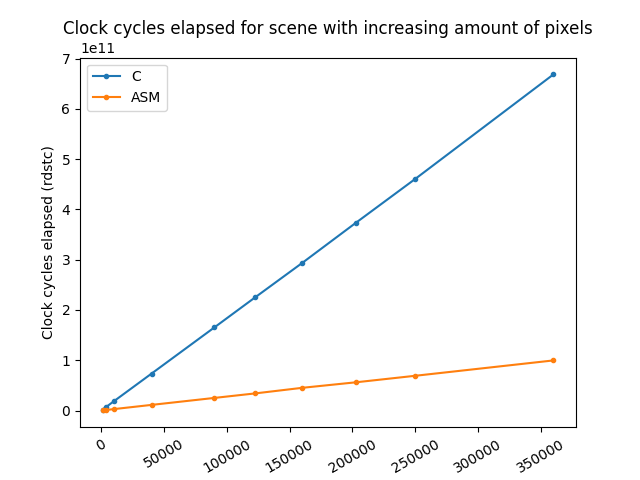
\includegraphics[width=\textwidth]{./imgs/exp2-res-line.png}
    \caption{Ciclos de clock por cantidad de píxeles}
    \label{fig:exp2-res-line}
  \end{subfigure}
  \caption{Resultado del experimento en 2 formatos}
  \label{fig:exp2-res}
\end{figure}

En la figura \ref{fig:exp2-res} podemos ver el resultado en 2 formatos. En
\ref{fig:exp2-res-bar} vemos como en cada resolución, RTASM requiere de muchos
menos ciclos para generar la misma imagen que RTC. Por otro lado, en
\ref{fig:exp2-res-line} se puede ver como estas magnitudes crecen de forma
lineal respecto a la cantidad de píxeles de cada imagen, lo cual tiene sentido.

\subsection{Ciclos de clock por tipo de objeto para distintas cantidades}

En este experimento, generaremos escenas de cubos, esferas y tetraedros, con una
cantidad creciente de elementos por escena.

Nuestro script \texttt{generate\_scenes.py} puede generar objetos de distintos
tamaños distribuidos en una cuadrícula y sus materiales correspondientes (como
se puede apreciar en el experimento anterior), y enfocar la cámara en el centro
para que todos los objetos sean visibles. Lo usaremos para generar escenas con
cuadrículas de $1 \times 1$, $2 \times 2$, hasta $10 \times 10$, compuestas
únicamente por cubos, esferas, o tetraedros.

Luego, mediremos la cantidad de ciclos de clock que le toma a cada ray tracer
generar la imagen realizando 5 mediciones y calculando el promedio.

\begin{figure}[H]
  \centering
  \begin{subfigure}[b]{0.45\textwidth}
    \centering
    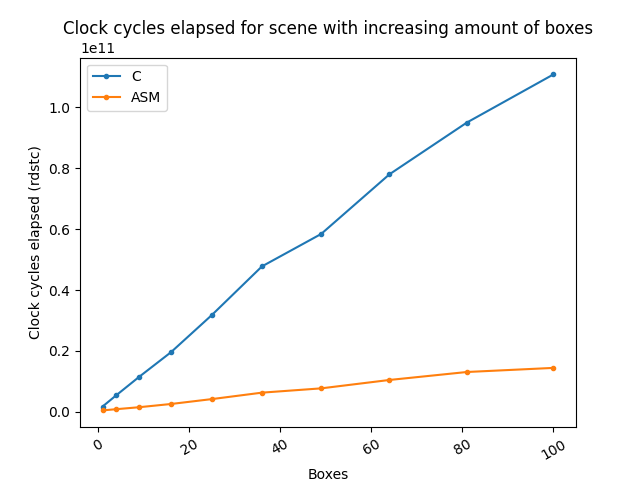
\includegraphics[width=\textwidth]{./imgs/exp3-box-c_vs_asm.png}
    \caption{Ciclos de clock por cantidad de \textit{boxes}}
  \end{subfigure}
  \hfill
  \begin{subfigure}[b]{0.45\textwidth}
    \centering
    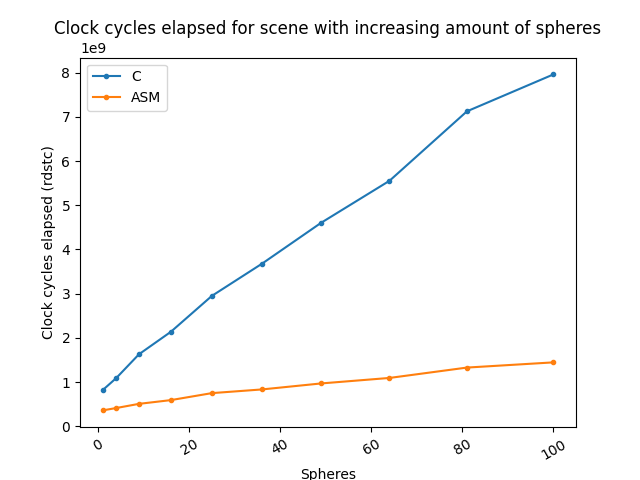
\includegraphics[width=\textwidth]{./imgs/exp3-sphere-c_vs_asm.png}
    \caption{Ciclos de clock por cantidad de \textit{spheres}}
  \end{subfigure}

  \begin{subfigure}[b]{0.45\textwidth}
    \centering
    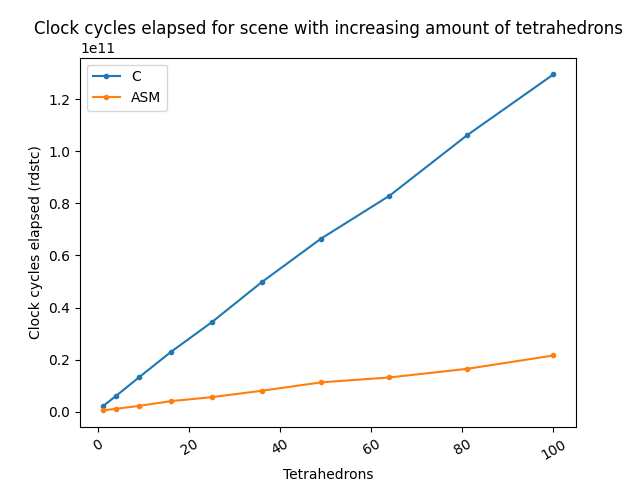
\includegraphics[width=\textwidth]{./imgs/exp3-tetra-c_vs_asm.png}
    \caption{Ciclos de clock por cantidad de \textit{tetrahedrons}}
  \end{subfigure}
  \caption{Resultados del experimento}
  \label{fig:exp3-res}
\end{figure}

En la figura \ref{fig:exp3-res} podemos ver los resultados por tipo de objeto.
En los 3 casos se puede ver un crecimiento casi lineal de la cantidad de ciclos,
tanto en RTC como en RTASM.

\subsection{Tiempo de ejecución entre C y ASM para mallas de triángulos}

En este experimento, comparamos la diferencia en el tiempo de ejecución que
tarda renderizar una imagen con un modelo de malla de triángulos. Se tomarán 10
mediciones del tiempo CPU, y se informará el promedio.

La escena a renderizar será la que se muestra en la figura \ref{fig:exp4-scene},
pero con una menor resolución para facilitar la medición.

\begin{figure}[H]
  \centering
  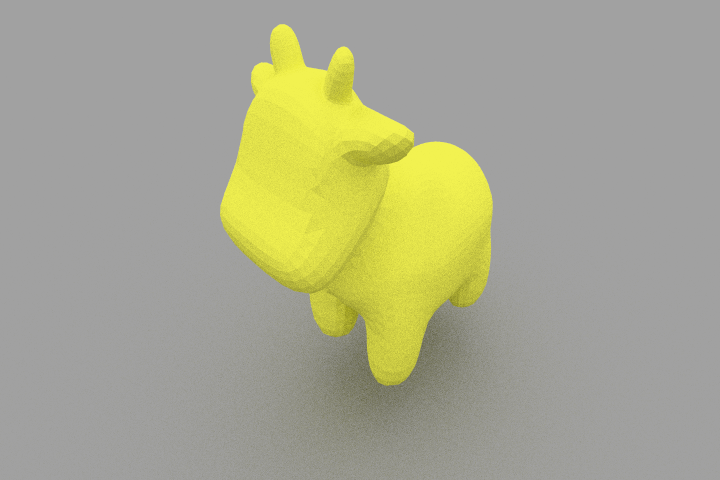
\includegraphics[width=.7\textwidth]{./imgs/exp4.png}
  \caption{Escena a utilizar en el experimento}
  \label{fig:exp4-scene}
\end{figure}

Nuevamente, RTASM obtiene un tiempo (8105.5ms) mucho menor al de RTC
(44836.1ms), que fue casi 5 veces más lento.
